\documentclass[a4paper,12pt]{report}

\newcommand{\nameInitial}{\textcolor{red}{D.H. von Eschwege}}
\newcommand{\nameFull}{\textcolor{red}{Daniel von Eschwege}}
\newcommand{\stNumber}{\textcolor{red}{21785155}}
\newcommand{\myDate}{\textcolor{red}{\today}}
\newcommand{\signature}{frontmatter/fig/Signature}


% Page layout
\usepackage[left=2.2cm,right=2.2cm,top=2.2cm,bottom=2.2cm]{geometry}

% Figures
\usepackage[margin=\the\parindent,small,bf,sf]{caption}
\usepackage{graphicx}
\usepackage[section]{placeins}
\usepackage{pdfpages}
\setlength{\abovecaptionskip}{7.5pt}  % spacing above and below captions
\newcommand*{\WaterMark}[2][0.2\paperwidth]{\AddToShipoutPicture*{\AtTextCenter{\parbox[c]{0pt}{\makebox[0pt][c]{\includegraphics[width=#1]{#2}}}}}}
\usepackage{subcaption}
 \usepackage{wrapfig}

% Font and text
\usepackage[afrikaans,english]{babel}
\usepackage{microtype}
\usepackage{setspace}
\usepackage{lmodern}
\newcommand{\myemph}[1]{{\sffamily\bfseries#1}}
\sloppy
\onehalfspacing
\usepackage{siunitx}
\usepackage{lipsum}


% Headings
\usepackage[raggedright,sf,bf]{titlesec}
\titlelabel{\thetitle.\ }
\titleformat{\chapter}[display]{\huge\bfseries\sffamily}{\chaptertitlename\ \thechapter}{15pt}{\raggedright}
% \titleformat{\chapter}[display]{\centering\huge\bfseries\sffamily}{\chaptertitlename\ \thechapter:}{15pt}{}
\titlespacing*{\chapter}{0pt}{0pt}{10pt}  % remove spacing before chapter headings

% Table of contents
\makeatletter
\let\originall@chapter\l@chapter
\def\l@chapter#1#2{\originall@chapter{{\sffamily #1}}{#2}}
\makeatother
\let \savenumberline \numberline
\def \numberline#1{\savenumberline{#1.}}

% Mathematics
\usepackage[cmex10]{amsmath}
\usepackage{amssymb}
\usepackage{cancel}
\DeclareMathOperator*{\argmax}{arg\,max}
\newcommand{\T}{^\textrm{T}}
\newcommand{\tr}{\textrm{tr}}
\renewcommand{\vec}[1]{\boldsymbol{\mathbf{#1}}}
\newcommand{\defeq}{\triangleq}

% Tables
\usepackage{booktabs}
\usepackage{tabularx}
\usepackage{multirow}
\newcommand{\mytable}{
    \centering
    \small
    \renewcommand{\arraystretch}{1.2}
    }
\renewcommand{\tabularxcolumn}[1]{m{#1}}
\newcolumntype{C}{>{\centering\arraybackslash}X}
\newcolumntype{L}{>{\raggedright\arraybackslash}X}

% Header and footer
\usepackage{fancyhdr}
\pagestyle{fancy}
\fancyhf{}
\renewcommand{\sectionmark}[1]{\markright{\normalsize \thesection.\ #1}}
\fancyhead[C]{\nouppercase{\textit{\rightmark}}}
\fancyhead[RO]{\thepage}
% \fancyhead[LE]{\thepage}  % double-sided printing
\fancyfoot{}
\setlength\headheight{14.5pt}
\renewcommand{\headrulewidth}{0pt}
\fancypagestyle{plain}{\fancyhead{}
                       \renewcommand{\headrulewidth}{0pt}
                       \fancyfoot[C]{\thepage}}

% Pseudo-code
\usepackage{algorithm}  % should go before \usepackage{hyperref}

% Table of contents and hyperlinks
\usepackage{hyperref}
\hypersetup{colorlinks=true,linktoc=all,citecolor=black,linkcolor=black}
\usepackage[nottoc]{tocbibind}

% Pseudo-code
\usepackage{algpseudocode}  % should go after \usepackage{hyperref}
\renewcommand{\thealgorithm}{\arabic{chapter}.\arabic{algorithm}} 
\captionsetup[algorithm]{labelfont={bf,sf},font=small,labelsep=colon}

% Bibliography
\usepackage{cite}  % automatically reorder inline citations
\bibliographystyle{IEEEtran}

% Fix titlesec issue
\usepackage{etoolbox}
\makeatletter
\patchcmd{\ttlh@hang}{\parindent\z@}{\parindent\z@\leavevmode}{}{}
\patchcmd{\ttlh@hang}{\noindent}{}{}{}
\makeatother

\setlength{\parindent}{0pt}

\begin{document}

% Front matter
\graphicspath{{frontmatter/fig/}}
\pagenumbering{Alph}

\begin{titlepage}
\begin{center}


\includegraphics[width=10cm]{USlogo-top}

\vfill

{\sffamily \bfseries \huge E344 Assignment 3 \par}

\vfill

{\large {\Large \nameFull} \\ \stNumber \par}

\vfill

\vfill

{Report submitted in partial fulfilment of the requirements of the module \\
Design (E) 344 for the degree Baccalaureus in Engineering in the Department of
Electrical and Electronic Engineering at Stellenbosch University. \par}

\vfill

%{\large {Supervisor}: Dr L. Skywalker} %\\
% Department of Electrical and Electronic Engineering \par}

\vfill

{\Large \myDate}
\end{center}
\end{titlepage}

\pagenumbering{roman}
%\chapter*{Declaration}
\newpage
\pagestyle{plain}
\addcontentsline{toc}{chapter}{Declaration}
\makeatletter\@mkboth{}{Declaration}\makeatother

\centerline{
\includegraphics[width=8cm]{USlogo-top}}
\vspace*{-10pt}

\section*{\centering Plagiaatverklaring / \textit{Plagiarism Declaration}}

\vspace*{5pt}

\begin{enumerate}
    \item Plagiaat is die oorneem en gebruik van die idees, materiaal en ander intellektuele eiendom van ander persone asof dit jou eie werk is.\\
    \textit{Plagiarism is the use of ideas, material and other intellectual property of another's work
        and to present is as my own.}
    
    \item Ek erken dat die pleeg van plagiaat 'n strafbare oortreding is aangesien dit 'n vorm van diefstal is.\\
    \textit{I agree that plagiarism is a punishable offence because it constitutes theft.}
    
    \item Ek verstaan ook dat direkte vertalings plagiaat is. \\
    \textit{I also understand that direct translations are plagiarism.}
    
    \item Dienooreenkomstig is alle aanhalings en bydraes vanuit enige bron (ingesluit die internet) volledig verwys (erken). Ek erken dat die woordelikse aanhaal van teks sonder aanhalingstekens (selfs al word die bron volledig erken) plagiaat is. \\
    \textit{Accordingly all quotations and contributions from any source whatsoever (including the internet) have been cited fully. I understand that the reproduction of text without quotation marks (even when the source is cited) is plagiarism}
    
    \item Ek verklaar dat die werk in hierdie skryfstuk vervat, behalwe waar anders aangedui, my eie oorspronklike werk is en dat ek dit nie vantevore in die geheel of gedeeltelik ingehandig het vir bepunting in hierdie module/werkstuk of 'n ander module/werkstuk~nie. \\
    \textit{I declare that the work contained in this assignment, except where otherwise stated, is my original work and that I have not previously (in its entirety or in part) submitted it for grading in this module/assignment or another module/assignment.}
\end{enumerate}

\vfill

\noindent \begin{tabularx}{1.0\linewidth}{|L|L|}
    \hline
    \hspace{2cm} \large{\stNumber}& \vspace{4mm}\hspace{2cm} \includegraphics[height=1.5cm]{\signature}\\

    \vspace{0mm}{Studentenommer / \textit{Student number}} & \vspace{0mm} {Handtekening / \textit{Signature}} \\
    \hline
    \vspace{1mm}  \hspace{2cm} \large{\nameInitial} & \vspace{1mm} \hspace{2cm} \large{\myDate }\\
    \vspace{1mm} {Voorletters en van / \textit{Initials and surname}} & \vspace{1mm} {Datum / \textit{Date}} \\
    \hline
\end{tabularx}

\vspace{15pt}




\tableofcontents
\listoffigures
\listoftables
\chapter*{Nomenclature\markboth{}{Nomenclature }}
\addcontentsline{toc}{chapter}{Nomenclature}


\textcolor{red}{update these}
% \vspace*{-3mm}
\subsubsection*{Variables and functions}

\begingroup
\renewcommand{\arraystretch}{1.2}
\renewcommand{\tabularxcolumn}[1]{p{#1}}
\begin{tabularx}{\textwidth}{@{}p{2.5cm}L}
    $p(x)$ & Probability density function with respect to variable $x$.\\
    $P(A)$ & Probability of event $A$ occurring.\\
    $\varepsilon$ & The Bayes error. \\
    $\varepsilon_u$ & The Bhattacharyya bound. \\
    $B$ & The Bhattacharyya distance. \\
    $s$ & An HMM state.  A subscript is used to refer to a particular state, e.g.\ $s_i$ refers to the $i^{\text{th}}$ state of an HMM. \\
    $\mathbf{S}$ & A set of HMM states. \\
    $\mathbf{F}$ & A set of frames. \\
    $\mathbf{o}_f$ & Observation (feature) vector associated with frame $f$. \\
    $\gamma_s(\mathbf{o}_f)$ & A posteriori probability of the observation vector $\mathbf{o}_f$ being generated by HMM state $s$. \\
    $\mu$ & Statistical mean vector. \\
    $\Sigma$ & Statistical covariance matrix. \\
    $L(\mathbf{S})$ & Log likelihood of the set of HMM states $\mathbf{S}$ generating the training set observation vectors assigned to the states in that set. \\
    $\mathcal{N}(\mathbf{x} | \mu, \Sigma)$ & Multivariate Gaussian PDF with mean $\mu$ and covariance matrix $\Sigma$.\\
    $a_{ij}$ & The probability of a transition from HMM state $s_i$ to state $s_j$. \\
    $N$ & Total number of frames or number of tokens, depending on the context. \\
    $D$ & Number of deletion errors. \\
    $I$ & Number of insertion errors. \\
    $S$ & Number of substitution errors. \\
\end{tabularx}
\endgroup


\newpage
\subsubsection*{Acronyms and abbreviations}
\textcolor{red}{update this}\\
\begingroup
\renewcommand{\arraystretch}{1.2}
\begin{tabular}{@{}p{2.5cm} l}
    AE      & Afrikaans English \\
    AID     & accent identification \\
    ASR     & automatic speech recognition \\
    AST     & African Speech Technology \\
    CE      & Cape Flats English \\
    DCD     & dialect-context-dependent \\
    DNN		& deep neural network \\
    G2P     & grapheme-to-phoneme \\
    GMM     & Gaussian mixture model \\
    HMM     & hidden Markov model \\
    HTK     & Hidden Markov Model Toolkit \\
    IE      & Indian South African English \\
    IPA     & International Phonetic Alphabet \\
    LM      & language model \\
    LMS     & language model scaling factor \\
    MFCC    & Mel-frequency cepstral coefficient \\
    MLLR    & maximum likelihood linear regression \\
    OOV     & out-of-vocabulary \\
    PD      & pronunciation dictionary \\
    PDF     & probability density function \\
    SAE     & South African English \\
    SAMPA   & Speech Assessment Methods Phonetic Alphabet \\
\end{tabular}
\endgroup

\newpage
\pagenumbering{arabic}

% Contents

\chapter{System design}
\section{System overview} \label{sec:system}

\begin{figure}[h]
    \centering
    \vspace{-0.7cm}
    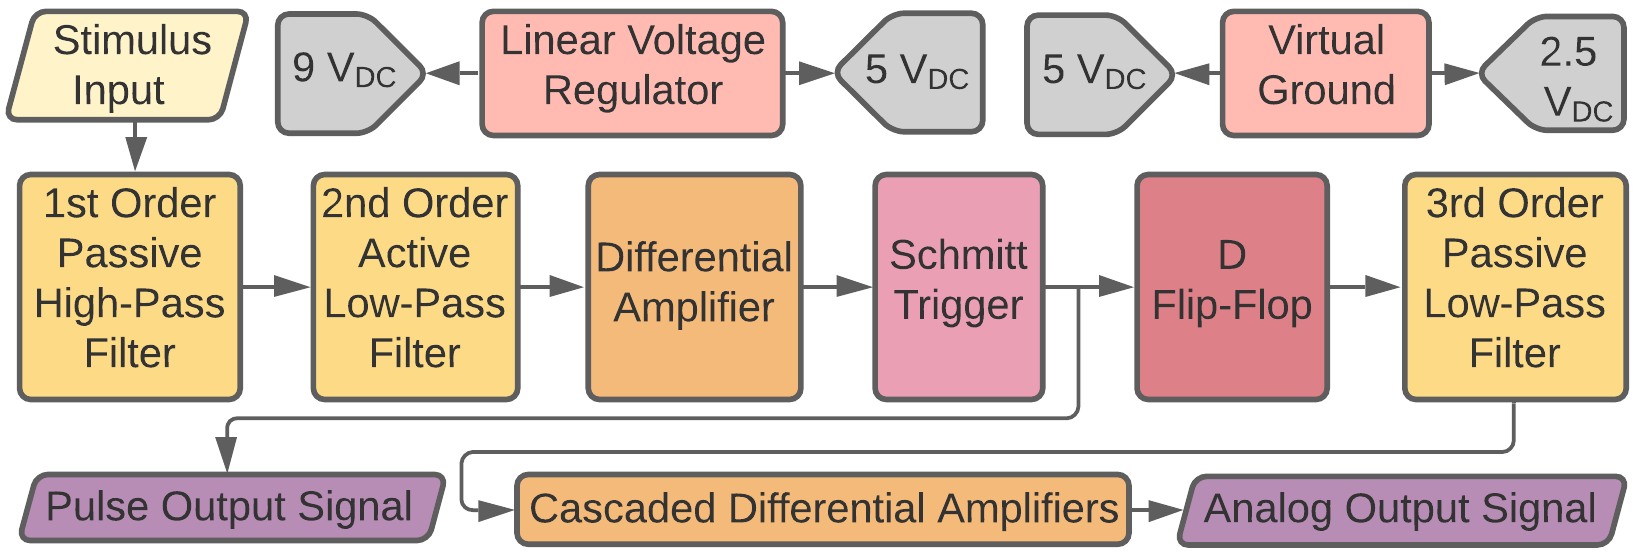
\includegraphics[width = 1\textwidth]{Figures/overview}
    \caption{System Diagram}
    \label{fig:overview}
\end{figure}

Creating a health monitoring system requires the design and implementation of a heart-rate sensor. This sensor obtains an input signal, from which pulses, corresponding to heart-beats are generated, as well as analogue values which represent the heart-rate. The aforementioned is achieved by means of various subcircuits, respectively responsible for voltage regulation, signal conditioning, pulse generation and conversion to analogue, which proceeds as can be seen in figure \ref{fig:overview} - explanation follows hereafter.
A voltage regulator generates 5 V which powers the circuit. See \ref{ } old report for the design. The stimulus input signal, obtained from the heart-rate sensor, is to be converted to a pulse output signal, but has an amplitude of insufficient magnitude, and is subject to high levels of noise. This necessitates signal conditioning: the input signal is fed into a first order passive high-pass filter and a second-order active low-pass filter consecutively, thereby attenuating both high- and low-frequency noise. The filters were chosen with maximal simplicity in mind, as to reduce cost and complexity, while still performing adequately. After filtering, the signal is amplified by means of a differential amplifier, resulting in a signal with a large amplitude and little noise. This allows for pulse generation by means of a Schmitt Trigger comparator, which produces an output pulse signal, where the frequency corresponds to the heart-rate. The Schmitt Trigger was preferred above alternatives as it provides a a noise margin by means of hysteresis, thereby eliminating heart-beat misdetections that otherwise arise. Further, an analogue voltage is required, where the voltage level represents the heart-rate. Filtering and peak detection using diodes was considered, but ultimately discarded, as diodes are non-linear, resulting in extremely slow simulation. Rather, the pulse output signal was converted to a pulse-width modulated signal, where the frequency of the former determined the duty cycle of the latter. This was done as PWM signals lend themselves to conversion-to-analogue by simple filtering. The PWM signal was obtained by using a D Flip-Flop in conjunction with a RC-circuit (see section \ref{•} for more detail), and was then filtered by a fourth-order passive RC filter. Passive components were selected as to reduce current usage and simulation time. The filter is of high order as to greatly minimize noise, as the settling time requirement for the analog signal was easily met.

\pagebreak


Also point the reader to your first report for more information on the temperature sensing and voltage regulation, and use a citation to it (add it to your \texttt{References.bib} file and cite it here). Remember to state what your remaining power budget is, based on Assignment 1's results. 










\chapter{System design}
\section{System overview} \label{sec:system}

\begin{figure}[h]
    \centering
    \vspace{-0.7cm}
    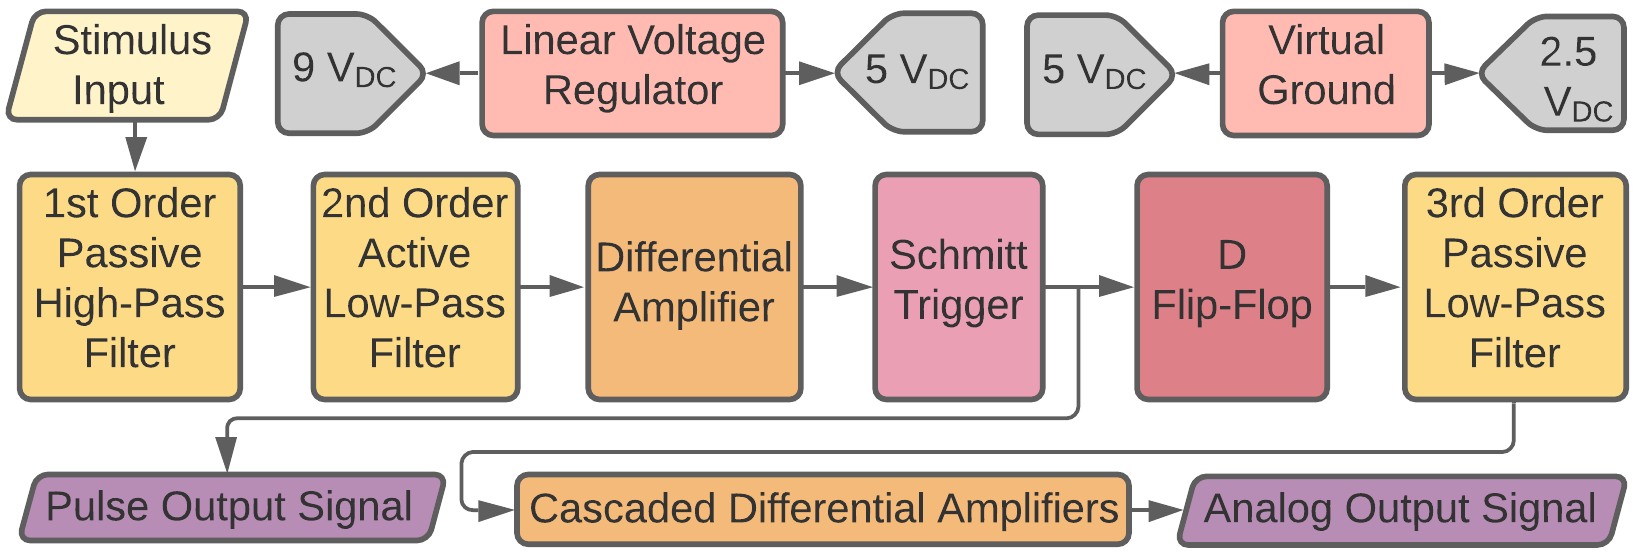
\includegraphics[width = 0.9\textwidth]{Figures/overview}
    \caption{System Diagram}
    \label{fig:overview}
\end{figure}


\chapter{Temperature sensor conditioning circuit}\label{sec:temp_sensor}

%**********************************************
\section{Intro} \label{sec:temp_intro}
%**********************************************
The signal obtained from the temperature sensor presents as DC, with a \SI{35}{\milli \volt}, \SI{50}{Hz} AC signal superimposed, which serves no purpose, but creates noise. The DC component increases linearly with respect to the temperature measured by the sensor. However, the sensor outputs a voltage of \SI{440}{\milli \volt} at 0\degree C, which increases by \SI{35}{\milli \volt} for every 1\degree C. These voltage levels are too small for a microcontroller ADC to take as input. Furthermore, as the sensor is only meant to measure human body temperature, the applicable range is only from 34\degree C to 42\degree C. The two aforementioned considerations necessitate amplification of the relevant part of the temperature sensor signal to occupy as much of a \numrange{0}{5} \si{\volt} range as possible, as this is the voltage range used by the ADC.
To this end, a temperature sensor conditioning circuit is required to transform the given input into the desired output. This conditioning circuit consists of a filter, an offset removing subcircuit, as well as an amplifier. The filter attenuates the AC signal present in the input signal in order to obtain an output signal with a minimal amount of noise. The offset removing subcircuit removes enough of the DC offset to ensure that the output signal is centered around \SI{2.5}{\volt}, which is necessary to obtain the largest possible output swing as discussed previously. Finally, the amplifier increases the magnitude of the input signal in order to be suitable as input for an ADC.

%**********************************************
\section{Design}\label{sec:temp_design}
%**********************************************
The amplifier was designed first, as its gain serves as the determining factor for the amount of noise reduction that is required from the filter. A TLC2272 op-amp was chosen as it allows for an output very close to its rails. Since the output signal has to be centered around \SI{2.5}{\volt}, a differential amplifier was decided upon, as the negative input can be used to adjust the offset present in the output. Given a zero-reference temperature sensor voltage ($V_{zero}$) of \SI{440}{\milli \volt}, with an increase ($V_{\Delta}$) of \SI{35}{\milli \volt} for every 1\degree C. Therefore, temperature sensor voltage levels are calculated as follows: $V_{temp} = V_{zero} + V_{\Delta} \times \mathrm{Temp}$ 

%Table \ref{tab:temp} shows some of the relevant voltage levels:

\begin{table}[h]
        \centering
        \footnotesize
        \caption{Temperatures and Corresponding Voltage Levels}
         \begin{tabular}{c@{\qquad}rrr}
          \toprule
          Temperature [\degree C] 	& 32    & 38	& 42\\
          Voltage [V] 			& 1.63	& 1.77	& 1.91\\
          \bottomrule
        \end{tabular}
     \label{tab:temp}
\end{table}

According to table \ref{tab:temp}, the maximum input voltage swing equals $1.91 - 1.63 = 0.28$V, and has a DC offset of \SI{1.77}{\volt}. Amplification is needed to reach an output voltage swing of \SI{5}{\volt}. Therefore:

$$A_v = \frac{V_{out}}{V_{in}} = \frac{5}{0.28} = 17.86$$

Considering the current design requirement of \SI{25}{mA} maximum, the input resistor R is selected as \SI{10}{\kilo \Omega}, which will therefore, at the highest possible voltage level (\SI{5}{\volt}), use \SI{0.5}{mA} of current.  This gives $R_{feedback} = 178.6$k$\Omega$, according to $A_v = \frac{{R}_{feedback}}{R}$ \cite{opamp}. R corresponds to $R_1$ and $R_2$, and $R_{feedback}$ to $R_{3}$ and $R_4$ in the final design diagram (figure \ref{fig:final}), which is shown here already to aid with the explanation of the design process. 

\begin{figure}[H]
    \centering
    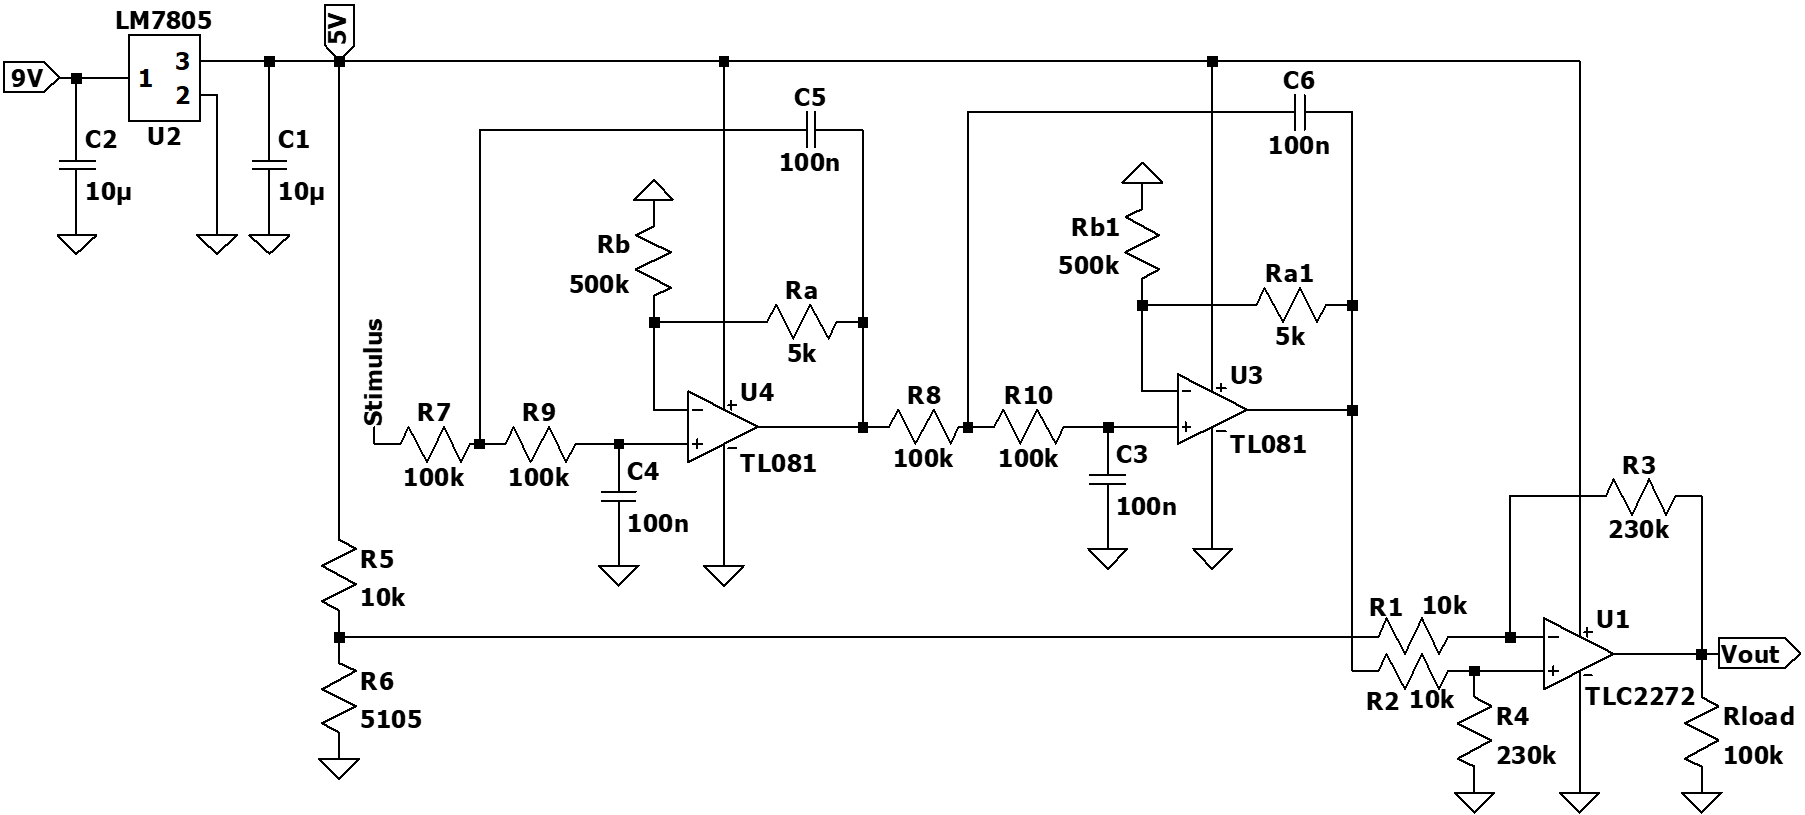
\includegraphics[width = 1\textwidth]{Figures/final.png}
    \caption{Temperature Sensor Circuit}
    \label{fig:final}
\end{figure}

Two points need to be considered: 
\begin{enumerate}
\item The DC offset of the input signal is undesired and has to be removed in order to obtain a zero-mean input signal. This can be achieved by designing another subcircuit that makes use of another op-amp, for example. This adds to the cost and complexity of the circuit.
\item The output signal has to be centered around \SI{2.5}{\volt}. This means that a DC offset has to be added in the form of a virtual ground.
\end{enumerate}

When considered in conjunction with each other, the DC offset alteration can be resolved in one step, thereby reducing cost and complexity significantly. The decision was therefore made to use a differential amplifier, with the input signal connected to the positive input, after which the voltage required at the negative input can be calculated in such a way as to simultaneously subtract the offset and add the virtual ground in one step, thereby producing an output DC offset of \SI{2.5}{\volt} (the lecturer mentions that this is an acceptable approach in Lecture Video 2).  This approach also simplifies the design procedure, as it becomes unnecessary to calculate the virtual ground separately. The differential amplifier, however, has to be non-inverting. The calculation thus reduces to a simple differential amplifier gain formula \cite{opamp}: 

$$V_{out}=\frac{{R}_{feedback}}{{R}}\left({V}_{in+}-{V}_{in-}\right) \;\;\; \rightarrow \;\;\; 2.5=\frac{178600}{10000}\left(1.77-{V}_{in-}\right)$$

With $V_{out}$ as \SI{2.5}{\volt}, $V_{in+}$ as \SI{1.77}{\volt} and the resistor values as calculated previously, ${V}_{in-} = 1.63 \; \mathrm{V}$. The voltage at ${V}_{in-}$ can be set by means of a voltage divider circuit, which takes \SI{5}{\volt} as input and is calculated as follows (resistor names in formulae are selected to conform with Figure \ref{fig:final}):

$${V}_{in-} = 5 (\frac{R_{6}}{R_{6}\times R_{5}})$$

Selecting $R_5$ as \SI{10}{\kilo \Omega} gives $R_6 =$ \SI{4.84}{\kilo \Omega}.\\

The filter has to be designed next. Possible design choices included an active/passive first order low-pass filter, a simple RC filter, or a second order low-pass filter. Simulation of the aforementioned filters has shown the following: the RC filter is very simple, but does not meet the design requirements w.r.t. noise. The passive low-pass filter is relatively simple, but does not meet the settling time requirement. The active low-pass filter meets both the noise and settling time requirements, but requires the TLC2272 op-amp to do so. Since a single TLC2272 op-amp is more expensive than multiple TL081 op-amps, the decision was made to rather use cascaded second order low-pass filters, which  make use of the TL081. This is somewhat more complex, but lowers the cost, as the final circuit now only uses three op-amps, two of which are the cheaper TL081 models. The cascaded setup also produces an output signal with extremely low noise.  A filter gain of close to unity is desired; for $R_A = $ \SI{500}{\kilo\Omega}, a value of \SI{5}{\kilo\Omega} is suitable for $R_A$, according to the formula from \cite{filter}:

$${A_v}=1+\frac{{R}_A}{R_B}$$

The settling time requirement of \SI{100}{ms} means that a cutoff frequency of more than \SI{10}{Hz} is needed, while the attenuation of noise requires a cutoff frequency below \SI{50}{Hz}. In order to minimize noise, the cutoff frequency was selected at \SI{15}{Hz} - the bandwidth thus also is \SI{15}{Hz} (only positive frequencies considered). Choosing R ($\mathrm{R_7 \; and \; R_9}$ in the diagram) as \SI{100}{\kilo\Omega} gives C ($\mathrm{C_4 \; and \; C_5}$) as \SI{106.1}{nF}, according to

$$f_c=\frac{1}{2 \pi RC}$$

The given cutoff frequency implies a rise time of \SI{19.1}{ms} according to $t_{r} \approx \frac{1.8}{w_{n}} = \frac{1.8}{2 \pi (15)}$\cite{cs}. This meets the requirement of \SI{100}{ms}. After design completion, this filter is then duplicated and connected back-to-back in order to form cascaded second-order low-pass filters, as seen in figure \ref{fig:final}.\\

Under most circumstances, it is a good design practice to include a unity gain op-amp at the input of the op-amp responsible for the correct offset, as it acts as a voltage buffer, thereby clamping the voltage against fluctuations caused by the differential amplifier's other input. This design practice was considered, but ultimately decided against, as tests with and without the buffer provided outputs of equal quality (similar to the output shown in section \ref{sec:temp_results}). The reason a buffer is not needed is due to the signal conditioning circuit already having a very high input resistance, following from the choice of resistors. The only notable differences resulting from the inclusion of a buffer were an increase in current drawn, as well as an increase in cost for the circuit components, as another op-amp is required. Therefore, in order to keep the current consumption below \SI{15}{mA}, as well as to use reduce cost by only using three op-amps, the voltage buffer was omitted in the final design. 


%**********************************************
\section{Results} \label{sec:temp_results}
%**********************************************
The designed circuit produces a signal centered at \SI{2.5}{\volt} with an output swing of \SI{4.86}{\volt} (figure \ref{fig:vout}), exceeding the required \SI{3.5}{\volt}. The absolute maximum amount of noise measured is \SI{25.6}{\milli\volt}, and the settling time is \SI{67}{ms}, thereby meeting the requirements of \SI{50}{\milli\volt} and \SI{100}{ms} respectively. Total current draw is \SI{12.83}{mA}, well below the required \SI{15}{mA}. The cutoff frequency, obtained via AC analysis simulation, is \SI{10.48}{Hz} (figure \ref{fig:ac}). Measurements and graphs of settling time, cutoff frequency and current drawn can be seen in Appendix C. It is thus clear that all requirements, as well as all bonus requirements, have been met with a good margin to spare, all the while using only three op-amps, two of which are the cheaper TL081 models. The output signal (light blue) is shown in figure \ref{fig:vout}.

\begin{figure}[h]
    \centering
    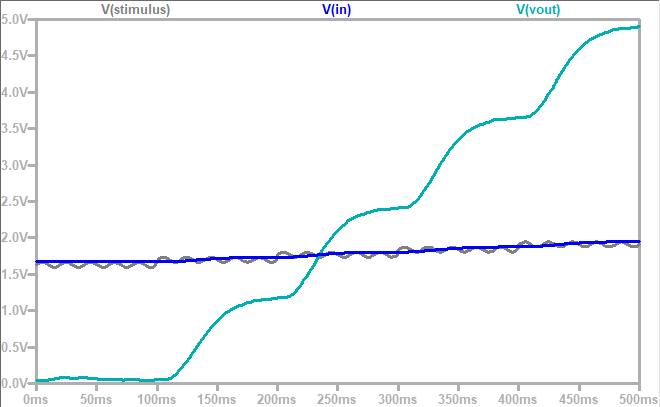
\includegraphics[width = 1\textwidth]{Figures/vout.png}
    \caption{Temperature Sensor Conditioning Circuit Output}
    \label{fig:vout}
\end{figure}

%**********************************************
\section{Summary}\label{sec:temp_summary}
%**********************************************
Concluding, the circuit performs very well, and successfully amplifies the temperature sensor output to a level that is readable by the microcontroller ADC, all the while attenuating almost all noise present in the input. The design is somewhat complex, but also cheaper, as it uses less of the TLC2272 op-amps.





% Bibliography
\bibliography{References}

% End matter
\appendix
\chapter{Social contract}
\makeatletter\@mkboth{}{Appendix}\makeatother
\label{appen:social_contract}
\textcolor{red}{Sign and inlcude.}
%     \begin{figure}[!htb]
%     \centering
%     	\fbox{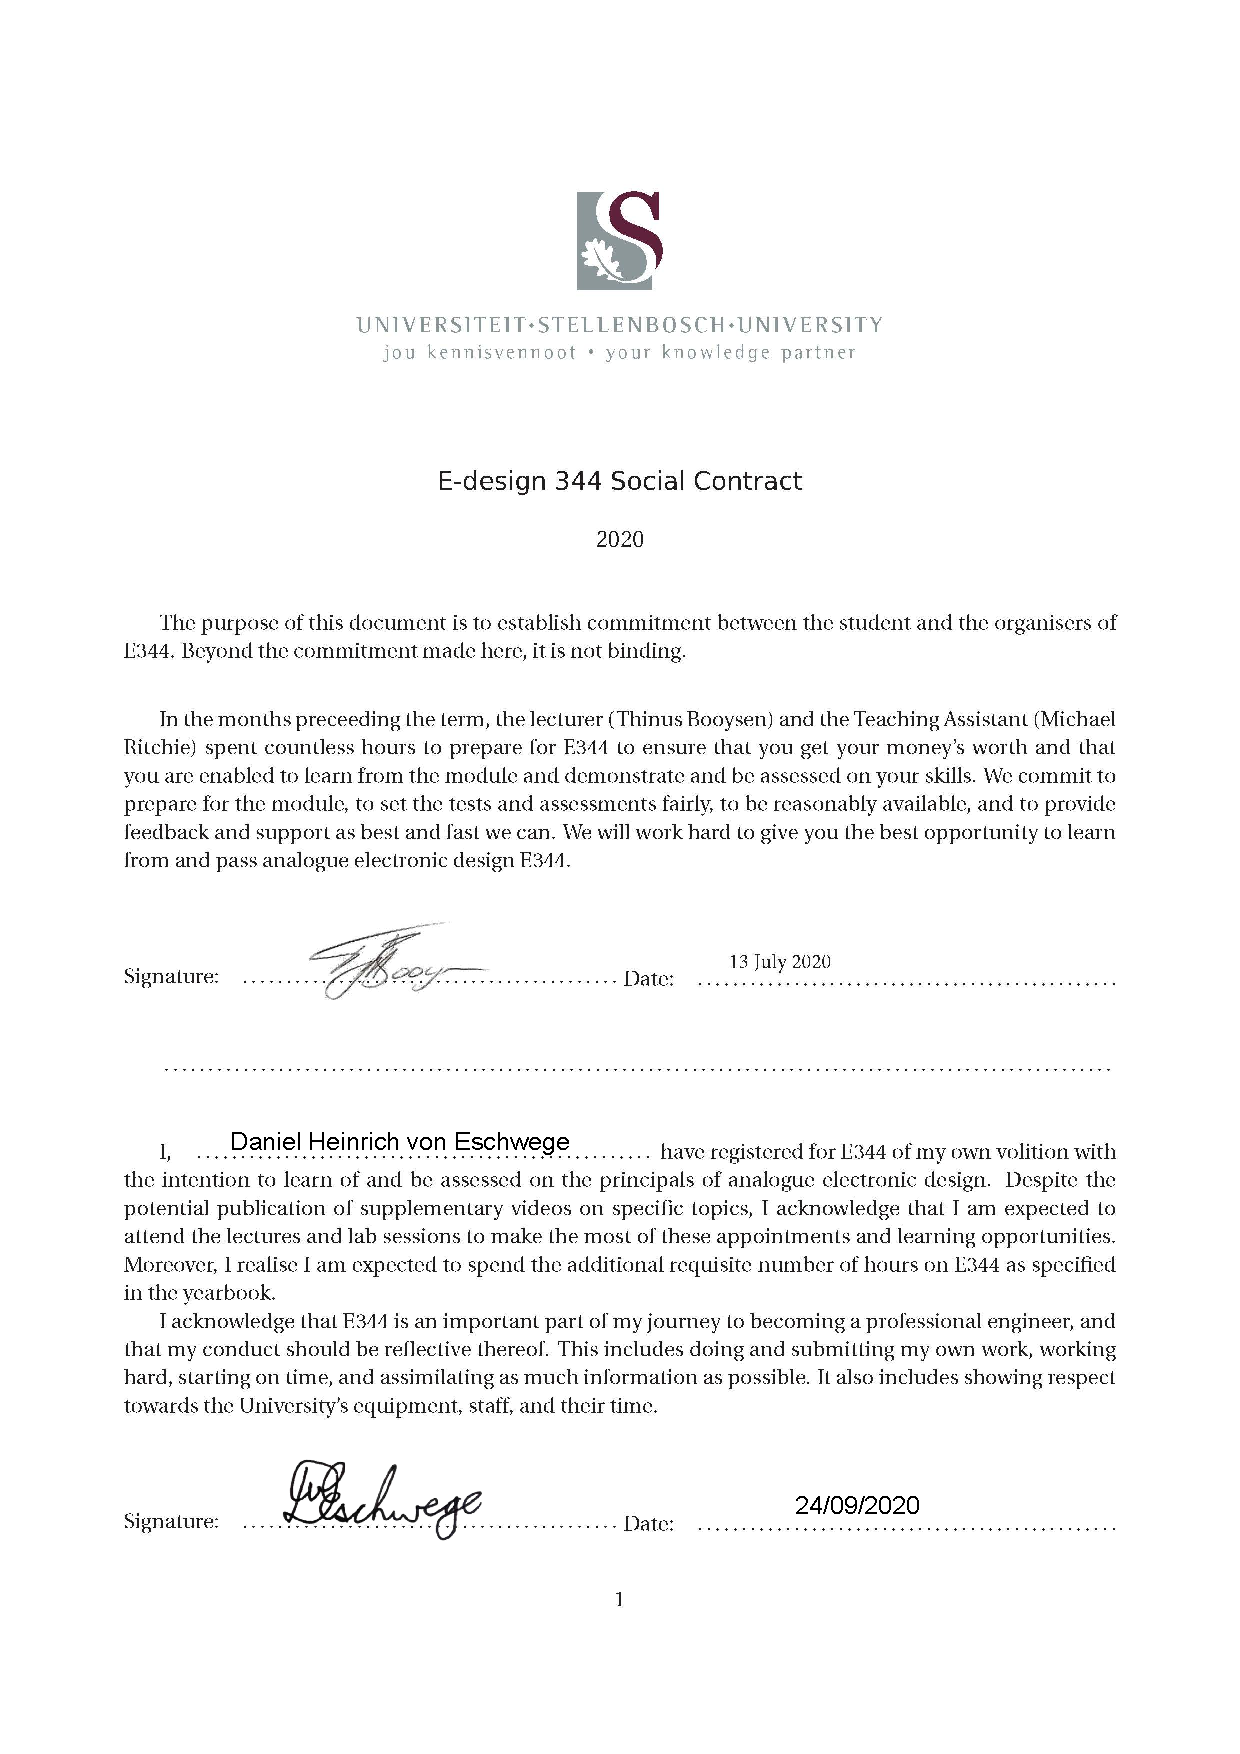
\includegraphics[width=0.78\linewidth]{./Figures/SocialContract_signed.pdf}}
%       \label{fig:social_contract}
%	\end{figure}
\chapter{GitHub Activity Heatmap}
\makeatletter\@mkboth{}{Appendix}\makeatother
\label{appen:github_heatmap}
\textcolor{red}{Take a screenshot of your github version control activity heatmap and insert here. }

     \begin{figure}[!htb]
     \centering
     	\fbox{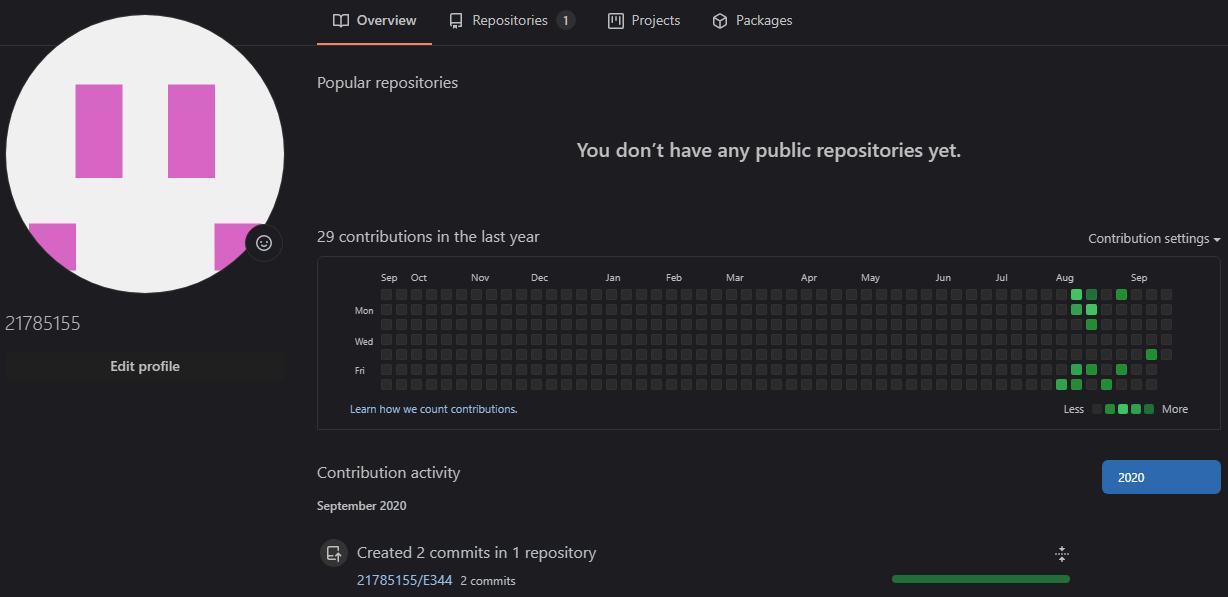
\includegraphics[width=1\linewidth]{./Figures/GitHub.png}}
	\label{fig:github}
	\end{figure}
     \chapter{Stuff you want to include}
R1 = \SI{500}{k\Omega}. $\tau = RC$. The capacitor charge oscillates between $V_L$ and $V_H$. $V_H =$ \SI{2.5}{V}. $V_L$ is reached for the first time at $t_{L_1}$ and $V_H$ at $t_{H_1}$. $V_L$ is then reached at  $t_{L_2}$. For \SI{150}{BPM} (or \SI{2.5}{Hz}), the pulse drives high for \SI{0.2}{ms}. Since the capacitor has to charge faster than \SI{0.2}{ms}, a charge time of \SI{0.16}{ms} was selected to add a 20\% margin, accounting for noise. Thus $t_{H_1} - t_{L_1} = 0.16$ and $t_{L_2} - t_{H_1} = 0.4 - 0.16 = 0.24$ for the 150 BPM signal. Finally,

$$V_L = 5\left(1-e^{\frac{t_{L_1}}{\tau}}\right)$$
$$V_H = 5\left(1-e^{\frac{-t_{H_1}}{\tau}}\right)$$
$$V_L = V_H\left(e^{\frac{t_{L_1}}{\tau}}\right)$$

giving $C = 1\mu$, when solving using the following MatLab script:\\

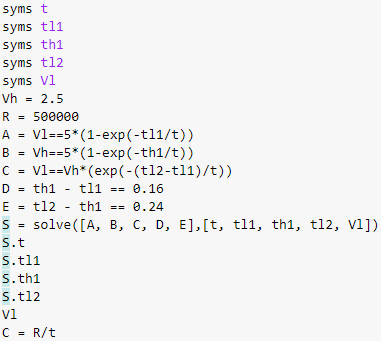
\includegraphics[width = 0.75\textwidth]{./Figures/script}

\end{document}

